% -*- coding: utf-8 -*-

\documentclass[10pt,dvipdfmx]{beamer}
\usepackage{tutorial}

\title{計算機実験(付録)}
\date{2019}

\begin{document}

\begin{frame}
  \titlepage
  \tableofcontents
\end{frame}

\section{実習その3}

\begin{frame}[t,fragile]{EX3-1: サンプルプログラムの実行}
  \begin{itemize}
    %\setlength{\itemsep}{1em}
  \item[3-1-1] ガウスの消去法のサンプルプログラム(\href{https://github.com/todo-group/computer-experiments/blob/master/exercise/linear_system/gauss.c}{exercise/linear\_system/gauss.c})をコンパイル・実行せよ。実行時にコマンドライン引数に行列の内容が書かれたファイル名({\tt input1.dat})を指定する必要があることに注意
\begin{lstlisting}
$ cc gauss.c -o gauss
$ ./gauss input1.dat
\end{lstlisting}
  \item[3-1-2] LU分解のサンプルプログラム(\href{https://github.com/todo-group/computer-experiments/blob/master/exercise/linear_system/lu_decomp.c}{exercise/linear\_system/lu\_decomp.c})をコンパイル・実行せよ。コンパイル時にLAPACKをリンク({\tt -llapack})する必要があることに注意(ハンドブック3.1.6節)
\begin{lstlisting}
$ cc lu_decomp.c -o lu_decomp -llapack
$ ./lu_decomp input1.dat
\end{lstlisting}
  \end{itemize}
\end{frame}

\begin{frame}[t,fragile]{EX3-2: ピボット選択、境界条件}
  \begin{itemize}
    %\setlength{\itemsep}{1em}
  \item[3-2-1] {\tt gauss.c}では、ピボット選択を行っていないため、入力が{\tt input2.dat}の場合には正しい解が得られない。ピボット選択を行うよう{\tt gauss.c}を修正せよ
  \item[3-2-2] \href{https://github.com/todo-group/computer-experiments/blob/master/exercise/linear_system/laplace_lu.c}{exercise/linear\_system/laplace\_lu.c}では、ディリクレ型の境界条件[$u(0,y) = \sin(\pi y)$, $u(x,0)=u(x,1)=u(1,y)=0$]のもとでのラプラス方程式の解をLU分解により求めている。境界条件を変えてみて解がどのように変化するか、Gnuplotを用いてプロットして確認せよ(Gnuplotの{\tt splot}コマンドを使う)
  \end{itemize}
\end{frame}

\begin{frame}[t,fragile]{EX3-3: ヤコビ法、ガウス・ザイデル法、SOR法}
  \begin{itemize}
    %\setlength{\itemsep}{1em}
  \item[3-3-1] \href{https://github.com/todo-group/computer-experiments/exercise/blob/master/linear_system/laplace_jacobi.c}{exercise/linear\_system/laplace\_jacobi.c}は、作りかけのヤコビ法のプログラムである。収束判定のコードを追加し、プログラムを完成せよ。計算結果や計算速度を{\tt laplace\_lu.c}と比較せよ
  \item[3-3-2] ヤコビ法のプログラム({\tt lapalace\_jacobi.c})を元に、ガウス・ザイデル法、SOR法のプログラムを作成せよ。収束までの回数を比較せよ。
特にSOR法の場合、パラメータ$\omega$の選び方により、どのように収束回数が変化するか観察し、最適な$\omega$の値について考察せよ
  \end{itemize}
\end{frame}

\section{代数方程式の解法}

\begin{frame}[t,fragile]{代数方程式}
  \begin{itemize}
    \setlength{\itemsep}{1em}
  \item 実係数の$n$次方程式
    \[
    P(z) = z^n + a_1 z^{n-1} + \cdots + a_n = 0
    \]
  \item ニュートン法 + 減次 (次数低下法)
    \begin{itemize}
    \item ニュートン法により一つの解($\alpha$)を求める
    \item $g(x) = f(x) / (x-\alpha)$の解として、他の解を逐次求めていく
    \item 毎回誤差がたまっていくため、解はくずれていく
    \end{itemize}
  \end{itemize}
\end{frame}


\begin{frame}[t,fragile]{Durand-Kerner-Aberth法 (Wierstrass法)}
  \begin{itemize}
    \setlength{\itemsep}{1em}
  \item 真の解を$\alpha_1,\alpha_2,\cdots,\alpha_n$とすると
    \[
    P(z) = (z-\alpha_1) (z-\alpha_2) \cdots (z-\alpha_n)
    \]
  \item $\alpha_1,\alpha_2,\cdots,\alpha_n$に現在の近似解$z^{(\nu)}_1,z^{(\nu)}_2,\cdots,z^{(\nu)}_n$を代入し、$z=z^{(\nu)}_k$における微分の値を評価
    \[
    P'(z^{(\nu)}_k) \approx \prod_{j \ne k} (z^{(\nu)}_k - z^{(\nu)}_j)
    \]
  \item ニュートン法による反復
    \[
    z^{(\nu+1)}_k = z^{(\nu)}_k - \frac{P(z^{(\nu)}_k)}{\prod_{j \ne k} (z^{(\nu)}_k - z^{(\nu)}_j)}
    \]
  \end{itemize}
\end{frame}

\begin{frame}[t,fragile]{初期値の選び方}
  \begin{itemize}
    \setlength{\itemsep}{1em}
  \item ある十分に大きな実数$r_0$を用いて
    \[
    z^{(0)}_k = - \frac{a_1}{n} + r_0 \exp \Big[ i \Big( \frac{2(k-1)\pi}{n} + \frac{\pi}{2n} \Big) \Big]
    \]
    複素平面上の中心$-a_1/n$、半径$r_0$の円周上の等間隔の点
  \item DKA法の収束
    \begin{itemize}
    \item $r_0$が十分大きい時
      \[\hspace*{-4cm} z^{(1)}_k + \frac{a_1}{n} \approx (1-\frac{1}{n}) (z^{(0)}_k + \frac{a_1}{n})
      \]
    \item 解の近傍では二次収束
    \item 解は互いに反発
    \item 例: $z^5-10z^4+43z^3-104z^2+150z-100=0$ (山本2003)
    \end{itemize}
  \end{itemize}
  \vspace*{-3.7cm}\hspace*{7.5cm}
  \resizebox{.3\textwidth}{!}{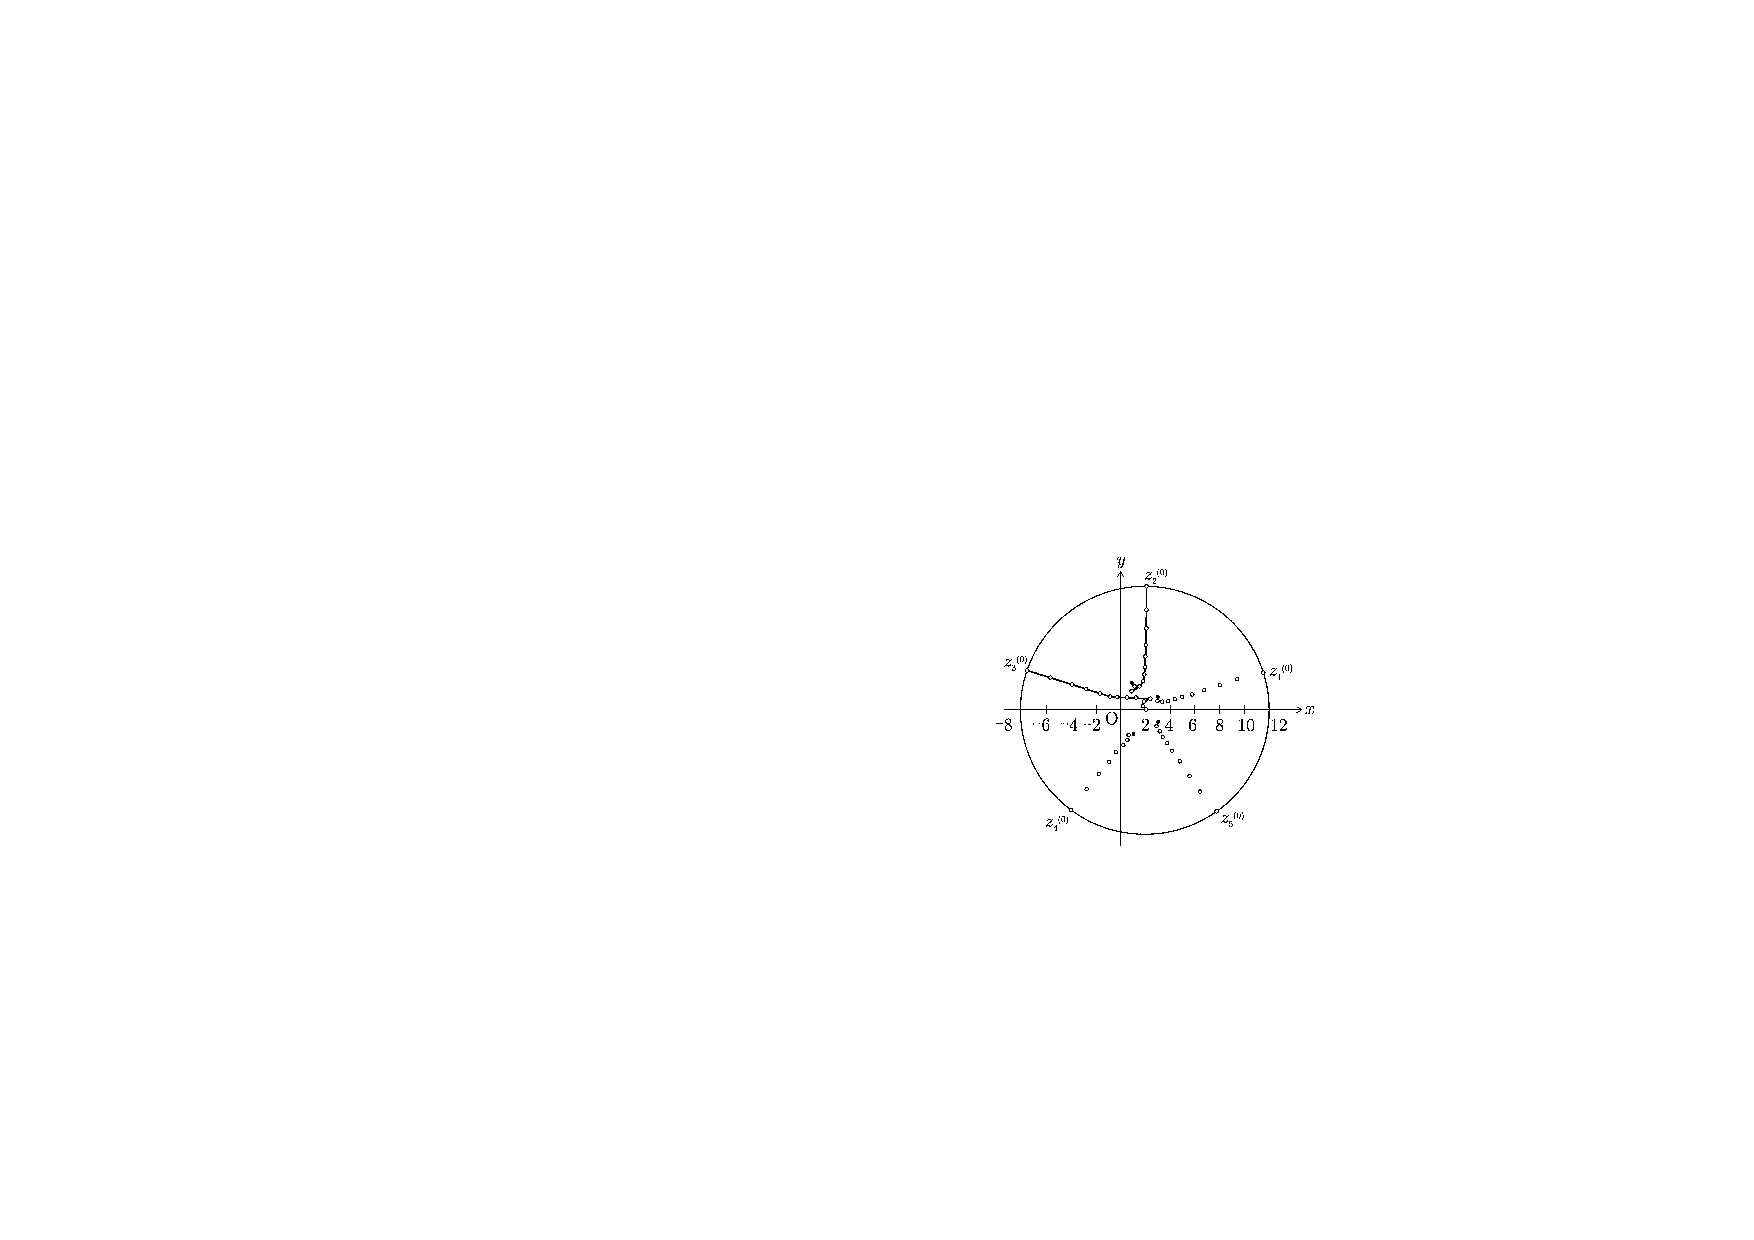
\includegraphics{image/DKA.pdf}}
\end{frame}

\section{実習その3}

\begin{frame}[t,fragile]{EX3-1: サンプルプログラムの実行}
  \begin{itemize}
    %\setlength{\itemsep}{1em}
  \item[3-1-1] ガウスの消去法のサンプルプログラム(\href{https://github.com/todo-group/computer-experiments/blob/master/exercise/linear_system/gauss.c}{exercise/linear\_system/gauss.c})をコンパイル・実行せよ。実行時にコマンドライン引数に行列の内容が書かれたファイル名({\tt input1.dat})を指定する必要があることに注意
\begin{lstlisting}
$ cc gauss.c -o gauss
$ ./gauss input1.dat
\end{lstlisting}
  \item[3-1-2] LU分解のサンプルプログラム(\href{https://github.com/todo-group/computer-experiments/blob/master/exercise/linear_system/lu_decomp.c}{exercise/linear\_system/lu\_decomp.c})をコンパイル・実行せよ。コンパイル時にLAPACKをリンク({\tt -llapack})する必要があることに注意(ハンドブック3.1.6節)
\begin{lstlisting}
$ cc lu_decomp.c -o lu_decomp -llapack
$ ./lu_decomp input1.dat
\end{lstlisting}
  \end{itemize}
\end{frame}

\begin{frame}[t,fragile]{EX3-2: ピボット選択、境界条件}
  \begin{itemize}
    %\setlength{\itemsep}{1em}
  \item[3-2-1] {\tt gauss.c}では、ピボット選択を行っていないため、入力が{\tt input2.dat}の場合には正しい解が得られない。ピボット選択を行うよう{\tt gauss.c}を修正せよ
  \item[3-2-2] \href{https://github.com/todo-group/computer-experiments/blob/master/exercise/linear_system/laplace_lu.c}{exercise/linear\_system/laplace\_lu.c}では、ディリクレ型の境界条件[$u(0,y) = \sin(\pi y)$, $u(x,0)=u(x,1)=u(1,y)=0$]のもとでのラプラス方程式の解をLU分解により求めている。境界条件を変えてみて解がどのように変化するか、Gnuplotを用いてプロットして確認せよ(Gnuplotの{\tt splot}コマンドを使う)
  \end{itemize}
\end{frame}

\begin{frame}[t,fragile]{EX3-3: ヤコビ法、ガウス・ザイデル法、SOR法}
  \begin{itemize}
    %\setlength{\itemsep}{1em}
  \item[3-3-1] \href{https://github.com/todo-group/computer-experiments/exercise/blob/master/linear_system/laplace_jacobi.c}{exercise/linear\_system/laplace\_jacobi.c}は、作りかけのヤコビ法のプログラムである。収束判定のコードを追加し、プログラムを完成せよ。計算結果や計算速度を{\tt laplace\_lu.c}と比較せよ
  \item[3-3-2] ヤコビ法のプログラム({\tt lapalace\_jacobi.c})を元に、ガウス・ザイデル法、SOR法のプログラムを作成せよ。収束までの回数を比較せよ。
特にSOR法の場合、パラメータ$\omega$の選び方により、どのように収束回数が変化するか観察し、最適な$\omega$の値について考察せよ
  \end{itemize}
\end{frame}

\section{実習その3}

\begin{frame}[t,fragile]{EX3-1: サンプルプログラムの実行}
  \begin{itemize}
    %\setlength{\itemsep}{1em}
  \item[3-1-1] ガウスの消去法のサンプルプログラム(\href{https://github.com/todo-group/computer-experiments/blob/master/exercise/linear_system/gauss.c}{exercise/linear\_system/gauss.c})をコンパイル・実行せよ。実行時にコマンドライン引数に行列の内容が書かれたファイル名({\tt input1.dat})を指定する必要があることに注意
\begin{lstlisting}
$ cc gauss.c -o gauss
$ ./gauss input1.dat
\end{lstlisting}
  \item[3-1-2] LU分解のサンプルプログラム(\href{https://github.com/todo-group/computer-experiments/blob/master/exercise/linear_system/lu_decomp.c}{exercise/linear\_system/lu\_decomp.c})をコンパイル・実行せよ。コンパイル時にLAPACKをリンク({\tt -llapack})する必要があることに注意(ハンドブック3.1.6節)
\begin{lstlisting}
$ cc lu_decomp.c -o lu_decomp -llapack
$ ./lu_decomp input1.dat
\end{lstlisting}
  \end{itemize}
\end{frame}

\begin{frame}[t,fragile]{EX3-2: ピボット選択、境界条件}
  \begin{itemize}
    %\setlength{\itemsep}{1em}
  \item[3-2-1] {\tt gauss.c}では、ピボット選択を行っていないため、入力が{\tt input2.dat}の場合には正しい解が得られない。ピボット選択を行うよう{\tt gauss.c}を修正せよ
  \item[3-2-2] \href{https://github.com/todo-group/computer-experiments/blob/master/exercise/linear_system/laplace_lu.c}{exercise/linear\_system/laplace\_lu.c}では、ディリクレ型の境界条件[$u(0,y) = \sin(\pi y)$, $u(x,0)=u(x,1)=u(1,y)=0$]のもとでのラプラス方程式の解をLU分解により求めている。境界条件を変えてみて解がどのように変化するか、Gnuplotを用いてプロットして確認せよ(Gnuplotの{\tt splot}コマンドを使う)
  \end{itemize}
\end{frame}

\begin{frame}[t,fragile]{EX3-3: ヤコビ法、ガウス・ザイデル法、SOR法}
  \begin{itemize}
    %\setlength{\itemsep}{1em}
  \item[3-3-1] \href{https://github.com/todo-group/computer-experiments/exercise/blob/master/linear_system/laplace_jacobi.c}{exercise/linear\_system/laplace\_jacobi.c}は、作りかけのヤコビ法のプログラムである。収束判定のコードを追加し、プログラムを完成せよ。計算結果や計算速度を{\tt laplace\_lu.c}と比較せよ
  \item[3-3-2] ヤコビ法のプログラム({\tt lapalace\_jacobi.c})を元に、ガウス・ザイデル法、SOR法のプログラムを作成せよ。収束までの回数を比較せよ。
特にSOR法の場合、パラメータ$\omega$の選び方により、どのように収束回数が変化するか観察し、最適な$\omega$の値について考察せよ
  \end{itemize}
\end{frame}

\section{実習その3}

\begin{frame}[t,fragile]{EX3-1: サンプルプログラムの実行}
  \begin{itemize}
    %\setlength{\itemsep}{1em}
  \item[3-1-1] ガウスの消去法のサンプルプログラム(\href{https://github.com/todo-group/computer-experiments/blob/master/exercise/linear_system/gauss.c}{exercise/linear\_system/gauss.c})をコンパイル・実行せよ。実行時にコマンドライン引数に行列の内容が書かれたファイル名({\tt input1.dat})を指定する必要があることに注意
\begin{lstlisting}
$ cc gauss.c -o gauss
$ ./gauss input1.dat
\end{lstlisting}
  \item[3-1-2] LU分解のサンプルプログラム(\href{https://github.com/todo-group/computer-experiments/blob/master/exercise/linear_system/lu_decomp.c}{exercise/linear\_system/lu\_decomp.c})をコンパイル・実行せよ。コンパイル時にLAPACKをリンク({\tt -llapack})する必要があることに注意(ハンドブック3.1.6節)
\begin{lstlisting}
$ cc lu_decomp.c -o lu_decomp -llapack
$ ./lu_decomp input1.dat
\end{lstlisting}
  \end{itemize}
\end{frame}

\begin{frame}[t,fragile]{EX3-2: ピボット選択、境界条件}
  \begin{itemize}
    %\setlength{\itemsep}{1em}
  \item[3-2-1] {\tt gauss.c}では、ピボット選択を行っていないため、入力が{\tt input2.dat}の場合には正しい解が得られない。ピボット選択を行うよう{\tt gauss.c}を修正せよ
  \item[3-2-2] \href{https://github.com/todo-group/computer-experiments/blob/master/exercise/linear_system/laplace_lu.c}{exercise/linear\_system/laplace\_lu.c}では、ディリクレ型の境界条件[$u(0,y) = \sin(\pi y)$, $u(x,0)=u(x,1)=u(1,y)=0$]のもとでのラプラス方程式の解をLU分解により求めている。境界条件を変えてみて解がどのように変化するか、Gnuplotを用いてプロットして確認せよ(Gnuplotの{\tt splot}コマンドを使う)
  \end{itemize}
\end{frame}

\begin{frame}[t,fragile]{EX3-3: ヤコビ法、ガウス・ザイデル法、SOR法}
  \begin{itemize}
    %\setlength{\itemsep}{1em}
  \item[3-3-1] \href{https://github.com/todo-group/computer-experiments/exercise/blob/master/linear_system/laplace_jacobi.c}{exercise/linear\_system/laplace\_jacobi.c}は、作りかけのヤコビ法のプログラムである。収束判定のコードを追加し、プログラムを完成せよ。計算結果や計算速度を{\tt laplace\_lu.c}と比較せよ
  \item[3-3-2] ヤコビ法のプログラム({\tt lapalace\_jacobi.c})を元に、ガウス・ザイデル法、SOR法のプログラムを作成せよ。収束までの回数を比較せよ。
特にSOR法の場合、パラメータ$\omega$の選び方により、どのように収束回数が変化するか観察し、最適な$\omega$の値について考察せよ
  \end{itemize}
\end{frame}

\section{実習その3}

\begin{frame}[t,fragile]{EX3-1: サンプルプログラムの実行}
  \begin{itemize}
    %\setlength{\itemsep}{1em}
  \item[3-1-1] ガウスの消去法のサンプルプログラム(\href{https://github.com/todo-group/computer-experiments/blob/master/exercise/linear_system/gauss.c}{exercise/linear\_system/gauss.c})をコンパイル・実行せよ。実行時にコマンドライン引数に行列の内容が書かれたファイル名({\tt input1.dat})を指定する必要があることに注意
\begin{lstlisting}
$ cc gauss.c -o gauss
$ ./gauss input1.dat
\end{lstlisting}
  \item[3-1-2] LU分解のサンプルプログラム(\href{https://github.com/todo-group/computer-experiments/blob/master/exercise/linear_system/lu_decomp.c}{exercise/linear\_system/lu\_decomp.c})をコンパイル・実行せよ。コンパイル時にLAPACKをリンク({\tt -llapack})する必要があることに注意(ハンドブック3.1.6節)
\begin{lstlisting}
$ cc lu_decomp.c -o lu_decomp -llapack
$ ./lu_decomp input1.dat
\end{lstlisting}
  \end{itemize}
\end{frame}

\begin{frame}[t,fragile]{EX3-2: ピボット選択、境界条件}
  \begin{itemize}
    %\setlength{\itemsep}{1em}
  \item[3-2-1] {\tt gauss.c}では、ピボット選択を行っていないため、入力が{\tt input2.dat}の場合には正しい解が得られない。ピボット選択を行うよう{\tt gauss.c}を修正せよ
  \item[3-2-2] \href{https://github.com/todo-group/computer-experiments/blob/master/exercise/linear_system/laplace_lu.c}{exercise/linear\_system/laplace\_lu.c}では、ディリクレ型の境界条件[$u(0,y) = \sin(\pi y)$, $u(x,0)=u(x,1)=u(1,y)=0$]のもとでのラプラス方程式の解をLU分解により求めている。境界条件を変えてみて解がどのように変化するか、Gnuplotを用いてプロットして確認せよ(Gnuplotの{\tt splot}コマンドを使う)
  \end{itemize}
\end{frame}

\begin{frame}[t,fragile]{EX3-3: ヤコビ法、ガウス・ザイデル法、SOR法}
  \begin{itemize}
    %\setlength{\itemsep}{1em}
  \item[3-3-1] \href{https://github.com/todo-group/computer-experiments/exercise/blob/master/linear_system/laplace_jacobi.c}{exercise/linear\_system/laplace\_jacobi.c}は、作りかけのヤコビ法のプログラムである。収束判定のコードを追加し、プログラムを完成せよ。計算結果や計算速度を{\tt laplace\_lu.c}と比較せよ
  \item[3-3-2] ヤコビ法のプログラム({\tt lapalace\_jacobi.c})を元に、ガウス・ザイデル法、SOR法のプログラムを作成せよ。収束までの回数を比較せよ。
特にSOR法の場合、パラメータ$\omega$の選び方により、どのように収束回数が変化するか観察し、最適な$\omega$の値について考察せよ
  \end{itemize}
\end{frame}

\section{カーネル法}

\begin{frame}[t,fragile]{カーネルトリック}
  \begin{itemize}
    %\setlength{\itemsep}{1em}
  \item 方程式を変形 ${\bf w} = \frac{1}{\lambda} \Phi^{\rm t} ({\bf y} -\Phi {\bf w})$
  \item $\alpha = \frac{1}{\lambda}({\bf y} -\Phi {\bf w})$と定義すると${\bf w} =\Phi^{\rm t} \alpha$
    \item $w$は$\begin{pmatrix} \phi_1(x_1) \\ \vdots \\ \phi_M(x_1) \end{pmatrix} \cdots 
      \begin{pmatrix} \phi_1(x_N) \\ \vdots \\ \phi_M(x_N) \end{pmatrix}$の線形結合
    \item $M$次元中の$N$次元部分空間にある ($M$: 基底関数の数、$N$: サンプル数)
    \item 基底関数を増やしても自由度は増えない
    \item $w$を求める代わりに、直接$\alpha$を求めても良い (リプリゼンター定理)
  \end{itemize}
\end{frame}

\begin{frame}[t,fragile]{カーネルによる線形回帰}
  \begin{itemize}
    %\setlength{\itemsep}{1em}
  \item 残差$R$を$\alpha$をつかって表現
    \[
    R(\alpha) = | y - \Phi \Phi^{\rm t} \alpha |^2 + \lambda \alpha^{\rm t} \Phi \Phi^{\rm t} \alpha
    \]
  \item グラム行列(Gram matrix) $K \equiv \Phi \Phi^{\rm t}$を導入すると
    \[
    R(\alpha) = | y - K \alpha |^2 + \lambda \alpha^{\rm t} K \alpha
    \]
  \item グラム行列($N \times N$対称行列)の成分
    \[
    K_{ik} = \sum_j \Phi_{ij} \Phi_{kj} = \sum_j \phi_j(x_i) \phi_j(x_k) \equiv {\color{red} k(x_i,x_k)}
    \]
  \item $M$個の基底関数の組を考えるかわりに1つのカーネル関数$k(x,x')$を導入すればよい(カーネル法)
  \end{itemize}
\end{frame}

\begin{frame}[t,fragile]{カーネルによる線形回帰}
  \begin{itemize}
    %\setlength{\itemsep}{1em}
  \item 残差$R$の最小化
    \[
    \alpha = (K + \lambda \, {\rm I})^{-1} {\bf y}
    \]
  \item 点$x$における$y$の推定値
    \begin{align*}
    y &= \sum_j \phi_j(x) w_j = \sum_{i,j} \phi_j(x) \phi_j(x_i) \alpha_i = \sum_i k(x_i,x) \alpha_i \\ &= k^{\rm t}(x) \alpha = k^{\rm t}(x) (K + \lambda \, {\rm I})^{-1} {\bf y}
k(x) = \begin{pmatrix} k(x_1,x) \\ k(x_2,x) \\ \vdots \\ k(x_N,x) \end{pmatrix}
    \end{align*}
  \item 例: ガウシアンカーネル $k(x,x') = \exp(-\beta|x-x'|^2)$
  \end{itemize}
\end{frame}

\section{ベイズ統計の基礎}

\begin{frame}[t,fragile]{条件付き確率}
  \begin{itemize}
    \setlength{\itemsep}{1em}
  \item 子供が二人いる家族において「二人の子供のうち少くとも一人が女の子である場合」二人とも女の子である確率は?
  \item 日本人の{\color{red} 1/10000}がウイルスAに感染しているとする。このウイルスに感染していると、{\color{red} 999/1000}の確率で検査で陽性となる。一方、感染していなくても、{\color{red} 1/100}の確率で陽性となってしまう(偽陽性)。検査結果が陽性の場合、感染している可能性は?
    \begin{itemize}
    \item 事象A:ウイルスに感染
    \item 事象B:検査で陽性
    \end{itemize}
  \end{itemize}
\end{frame}

\begin{frame}[t,fragile]{ベイズの定理}
  \begin{itemize}
    %\setlength{\itemsep}{1em}
  \item 確率に対する公式
    \begin{align*}
      P(A \cap B) &= P(B|A) P(A) = P(A|B) P(B) \\ P(B) &= P(B|A) P(A) + P(B|\bar{A}) P(\bar{A})
    \end{align*}
  \item ベイズの定理 (確率の反転)
    \[
    P(A|B) = \frac{P(B|A)P(A)}{P(B)} = \frac{P(B|A)P(A)}{P(B|A) P(A) + P(B|\bar{A}) P(\bar{A})}
    \]
  \item 検査が陽性でも、実際に感染している可能性(確率)は
    \[
    \frac{\frac{999}{1000} \cdot \frac{1}{10000}}{\frac{999}{1000} \cdot \frac{1}{10000} + \frac{1}{100} \cdot \frac{9999}{10000}} \approx {\color{red} 0.009}
    \]
    \begin{itemize}
    \item 予想よりずっと小さい?
    \item 「検査が陽性」という事実により、感染している確率が 0.01\%から 0.9\%に増加 $\Rightarrow$ ベイズ統計・機械学習の基礎公式
    \end{itemize}
  \end{itemize}
\end{frame}

\begin{frame}[t,fragile]{ベイズ統計学(Bayesian Statistics)}
  \begin{itemize}
    %\setlength{\itemsep}{1em}
  \item 条件つき確率におけるベイズの定理
    \[
    p(\theta|y) \sim p(y|\theta) p(\theta)
    \]
  \item この(あたりまえの)関係式をベイズ統計では以下のように解釈する
    \begin{itemize}
    \item $\theta$未知母数(パラメータ) : 物理量の平均、分散、比例係数、etc
    (確定した値ではなくある分布に従って変動する量として考える)
    \item $y$ 観測値 : すでに「与えられた」確定したものと考える
    \item $p(\theta)$ 事前確率 (prior probability) : 母数に関する何らかの事前情報
    \item $p(y|\theta)$ 尤度 (likelihood) : $y$は与えられている$\theta$の関数と解釈。$l(\theta|y)$ と書く
    \item $p(\theta|y)$ 事後確率 (posterior probability) : 観測で情報が増えた後の$\theta$の確率分布
    \end{itemize}
  \end{itemize}
\end{frame}

\begin{frame}[t,fragile]{頻度主義的アプローチとベイズ的アプローチ}
  \begin{itemize}
    %\setlength{\itemsep}{1em}
  \item コインを一回投げて表が出る確率 $q$
  \item 連続して三回連続して表が出る($y$)確率 $p(y|q) = q^3 = l(q|y)$  ($q$ の尤度関数)
  \item 頻度主義的アプローチ(最尤推定)
    \begin{itemize}
    \item $q$ の推定値 $q=1$ \ \ $\Rightarrow$ \ \ 未来永劫表が出続ける!
    \item 観測データ数$\sim$母数の数の時 \ \ $\Rightarrow$ \ \ 過学習(over-fitting)
    \end{itemize}
  \item ベイズ的アプローチ
    \begin{itemize}
    \item $q$の事前分布として $p(q) = 1$  \ \ $\Rightarrow$ \ \ %事後分布
      $p(q|y) \sim l(q|y) p(q) = q^3$
    \end{itemize}
  \item ベイズ的アプローチでは過学習の問題が生じない
  \item 有効パラメータ数が自動的にデータ集合のサイズに適合
  \end{itemize}
\end{frame}

\begin{frame}[t,fragile]{回帰分析への応用}
  \begin{itemize}
    %\setlength{\itemsep}{1em}
  \item 単回帰モデル: $y=a+bx+\epsilon$ \ \ ($\epsilon$: ノイズ)
  \item 尤度関数 (likelihood function) :
    \[
    l(a, b | \{x_i\}, \{y_i\}) = p(\{y_i\} | \{x_i\}, a, b) \sim \prod_i \exp \Big[ -\frac{(y_i - (a+bx_i))^2}{2\sigma^2}\Big]
    \]
  \item 事前分布を導入
    \begin{itemize}
    \item 例えば $a$, $b$ について ${\cal N}(0,1000)$
    \end{itemize}
  \item 事後分布:
    \[
    p(a,b | \{x_i\}, \{y_i\}) \sim l(a, b | \{x_i\}, \{y_i\}) p(a) p(b)
    \]
    \begin{itemize}
      \item $a$, $b$ の事後周辺分布から期待値とその確からしさを推定
      \item 最大事後確率(MAP)推定
    \end{itemize}
  \end{itemize}
\end{frame}

\begin{frame}[t,fragile]{最小二乗法・カーネル法・ベイズ推定}
  \begin{itemize}
    \setlength{\itemsep}{1em}
  \item 非線形最小二乗法
    \begin{itemize}
    \item 非線形の最小化問題
    \end{itemize}
  \item カーネル法
    \begin{itemize}
    \item 実質的に無限次元の問題を解くことができる
    \item データサイズが大きくなるとその3乗に比例して計算量が増大
    \end{itemize}
  \item ベイズ推定
    \begin{itemize}
    \item 事後確率をコンパクトな形で求めることは難しい
    \item モンテカルロ法の利用
    \end{itemize}    
  \end{itemize}
\end{frame}

\section{実習その3}

\begin{frame}[t,fragile]{EX3-1: サンプルプログラムの実行}
  \begin{itemize}
    %\setlength{\itemsep}{1em}
  \item[3-1-1] ガウスの消去法のサンプルプログラム(\href{https://github.com/todo-group/computer-experiments/blob/master/exercise/linear_system/gauss.c}{exercise/linear\_system/gauss.c})をコンパイル・実行せよ。実行時にコマンドライン引数に行列の内容が書かれたファイル名({\tt input1.dat})を指定する必要があることに注意
\begin{lstlisting}
$ cc gauss.c -o gauss
$ ./gauss input1.dat
\end{lstlisting}
  \item[3-1-2] LU分解のサンプルプログラム(\href{https://github.com/todo-group/computer-experiments/blob/master/exercise/linear_system/lu_decomp.c}{exercise/linear\_system/lu\_decomp.c})をコンパイル・実行せよ。コンパイル時にLAPACKをリンク({\tt -llapack})する必要があることに注意(ハンドブック3.1.6節)
\begin{lstlisting}
$ cc lu_decomp.c -o lu_decomp -llapack
$ ./lu_decomp input1.dat
\end{lstlisting}
  \end{itemize}
\end{frame}

\begin{frame}[t,fragile]{EX3-2: ピボット選択、境界条件}
  \begin{itemize}
    %\setlength{\itemsep}{1em}
  \item[3-2-1] {\tt gauss.c}では、ピボット選択を行っていないため、入力が{\tt input2.dat}の場合には正しい解が得られない。ピボット選択を行うよう{\tt gauss.c}を修正せよ
  \item[3-2-2] \href{https://github.com/todo-group/computer-experiments/blob/master/exercise/linear_system/laplace_lu.c}{exercise/linear\_system/laplace\_lu.c}では、ディリクレ型の境界条件[$u(0,y) = \sin(\pi y)$, $u(x,0)=u(x,1)=u(1,y)=0$]のもとでのラプラス方程式の解をLU分解により求めている。境界条件を変えてみて解がどのように変化するか、Gnuplotを用いてプロットして確認せよ(Gnuplotの{\tt splot}コマンドを使う)
  \end{itemize}
\end{frame}

\begin{frame}[t,fragile]{EX3-3: ヤコビ法、ガウス・ザイデル法、SOR法}
  \begin{itemize}
    %\setlength{\itemsep}{1em}
  \item[3-3-1] \href{https://github.com/todo-group/computer-experiments/exercise/blob/master/linear_system/laplace_jacobi.c}{exercise/linear\_system/laplace\_jacobi.c}は、作りかけのヤコビ法のプログラムである。収束判定のコードを追加し、プログラムを完成せよ。計算結果や計算速度を{\tt laplace\_lu.c}と比較せよ
  \item[3-3-2] ヤコビ法のプログラム({\tt lapalace\_jacobi.c})を元に、ガウス・ザイデル法、SOR法のプログラムを作成せよ。収束までの回数を比較せよ。
特にSOR法の場合、パラメータ$\omega$の選び方により、どのように収束回数が変化するか観察し、最適な$\omega$の値について考察せよ
  \end{itemize}
\end{frame}

\section{実習その3}

\begin{frame}[t,fragile]{EX3-1: サンプルプログラムの実行}
  \begin{itemize}
    %\setlength{\itemsep}{1em}
  \item[3-1-1] ガウスの消去法のサンプルプログラム(\href{https://github.com/todo-group/computer-experiments/blob/master/exercise/linear_system/gauss.c}{exercise/linear\_system/gauss.c})をコンパイル・実行せよ。実行時にコマンドライン引数に行列の内容が書かれたファイル名({\tt input1.dat})を指定する必要があることに注意
\begin{lstlisting}
$ cc gauss.c -o gauss
$ ./gauss input1.dat
\end{lstlisting}
  \item[3-1-2] LU分解のサンプルプログラム(\href{https://github.com/todo-group/computer-experiments/blob/master/exercise/linear_system/lu_decomp.c}{exercise/linear\_system/lu\_decomp.c})をコンパイル・実行せよ。コンパイル時にLAPACKをリンク({\tt -llapack})する必要があることに注意(ハンドブック3.1.6節)
\begin{lstlisting}
$ cc lu_decomp.c -o lu_decomp -llapack
$ ./lu_decomp input1.dat
\end{lstlisting}
  \end{itemize}
\end{frame}

\begin{frame}[t,fragile]{EX3-2: ピボット選択、境界条件}
  \begin{itemize}
    %\setlength{\itemsep}{1em}
  \item[3-2-1] {\tt gauss.c}では、ピボット選択を行っていないため、入力が{\tt input2.dat}の場合には正しい解が得られない。ピボット選択を行うよう{\tt gauss.c}を修正せよ
  \item[3-2-2] \href{https://github.com/todo-group/computer-experiments/blob/master/exercise/linear_system/laplace_lu.c}{exercise/linear\_system/laplace\_lu.c}では、ディリクレ型の境界条件[$u(0,y) = \sin(\pi y)$, $u(x,0)=u(x,1)=u(1,y)=0$]のもとでのラプラス方程式の解をLU分解により求めている。境界条件を変えてみて解がどのように変化するか、Gnuplotを用いてプロットして確認せよ(Gnuplotの{\tt splot}コマンドを使う)
  \end{itemize}
\end{frame}

\begin{frame}[t,fragile]{EX3-3: ヤコビ法、ガウス・ザイデル法、SOR法}
  \begin{itemize}
    %\setlength{\itemsep}{1em}
  \item[3-3-1] \href{https://github.com/todo-group/computer-experiments/exercise/blob/master/linear_system/laplace_jacobi.c}{exercise/linear\_system/laplace\_jacobi.c}は、作りかけのヤコビ法のプログラムである。収束判定のコードを追加し、プログラムを完成せよ。計算結果や計算速度を{\tt laplace\_lu.c}と比較せよ
  \item[3-3-2] ヤコビ法のプログラム({\tt lapalace\_jacobi.c})を元に、ガウス・ザイデル法、SOR法のプログラムを作成せよ。収束までの回数を比較せよ。
特にSOR法の場合、パラメータ$\omega$の選び方により、どのように収束回数が変化するか観察し、最適な$\omega$の値について考察せよ
  \end{itemize}
\end{frame}

\section{スーパーコンピューターと計算物理}

\begin{frame}[t,fragile]{計算機の進化}
  \begin{itemize}
    \setlength{\itemsep}{1em}
  \item 計算機の性能は指数関数的に伸び続けている
    \begin{itemize}
    \item 1年で1.9倍 ⇒ 4年で10倍 ⇒ 過去70年間で100兆倍
    \item 世界初のスパコンCray-1 (1976年)の演算性能 約160MFlops
    \item iPhone6 (2014年)の演算性能 約900MFlops
    \item 2020年代初頭には、1EFlops (エクサフロップス)へ
    \end{itemize}
  \item 現代のスーパーコンピュータは全て
    \begin{itemize}
      \item 並列コンピュータ (CPU数 1,000〜100,000)
      \item マルチコア or メニーコア (CPUあたりのコア数 8 〜 1,000)
      \item 多層にわたる階層構造
      \item 演算に比べて、データを移動するコストの方が高い
    \end{itemize}
  \end{itemize}
\end{frame}

\section{並列計算とは}

\begin{frame}[t,fragile]{Richardson's Forecast Factory (1922)}
  \resizebox{.8\textwidth}{!}{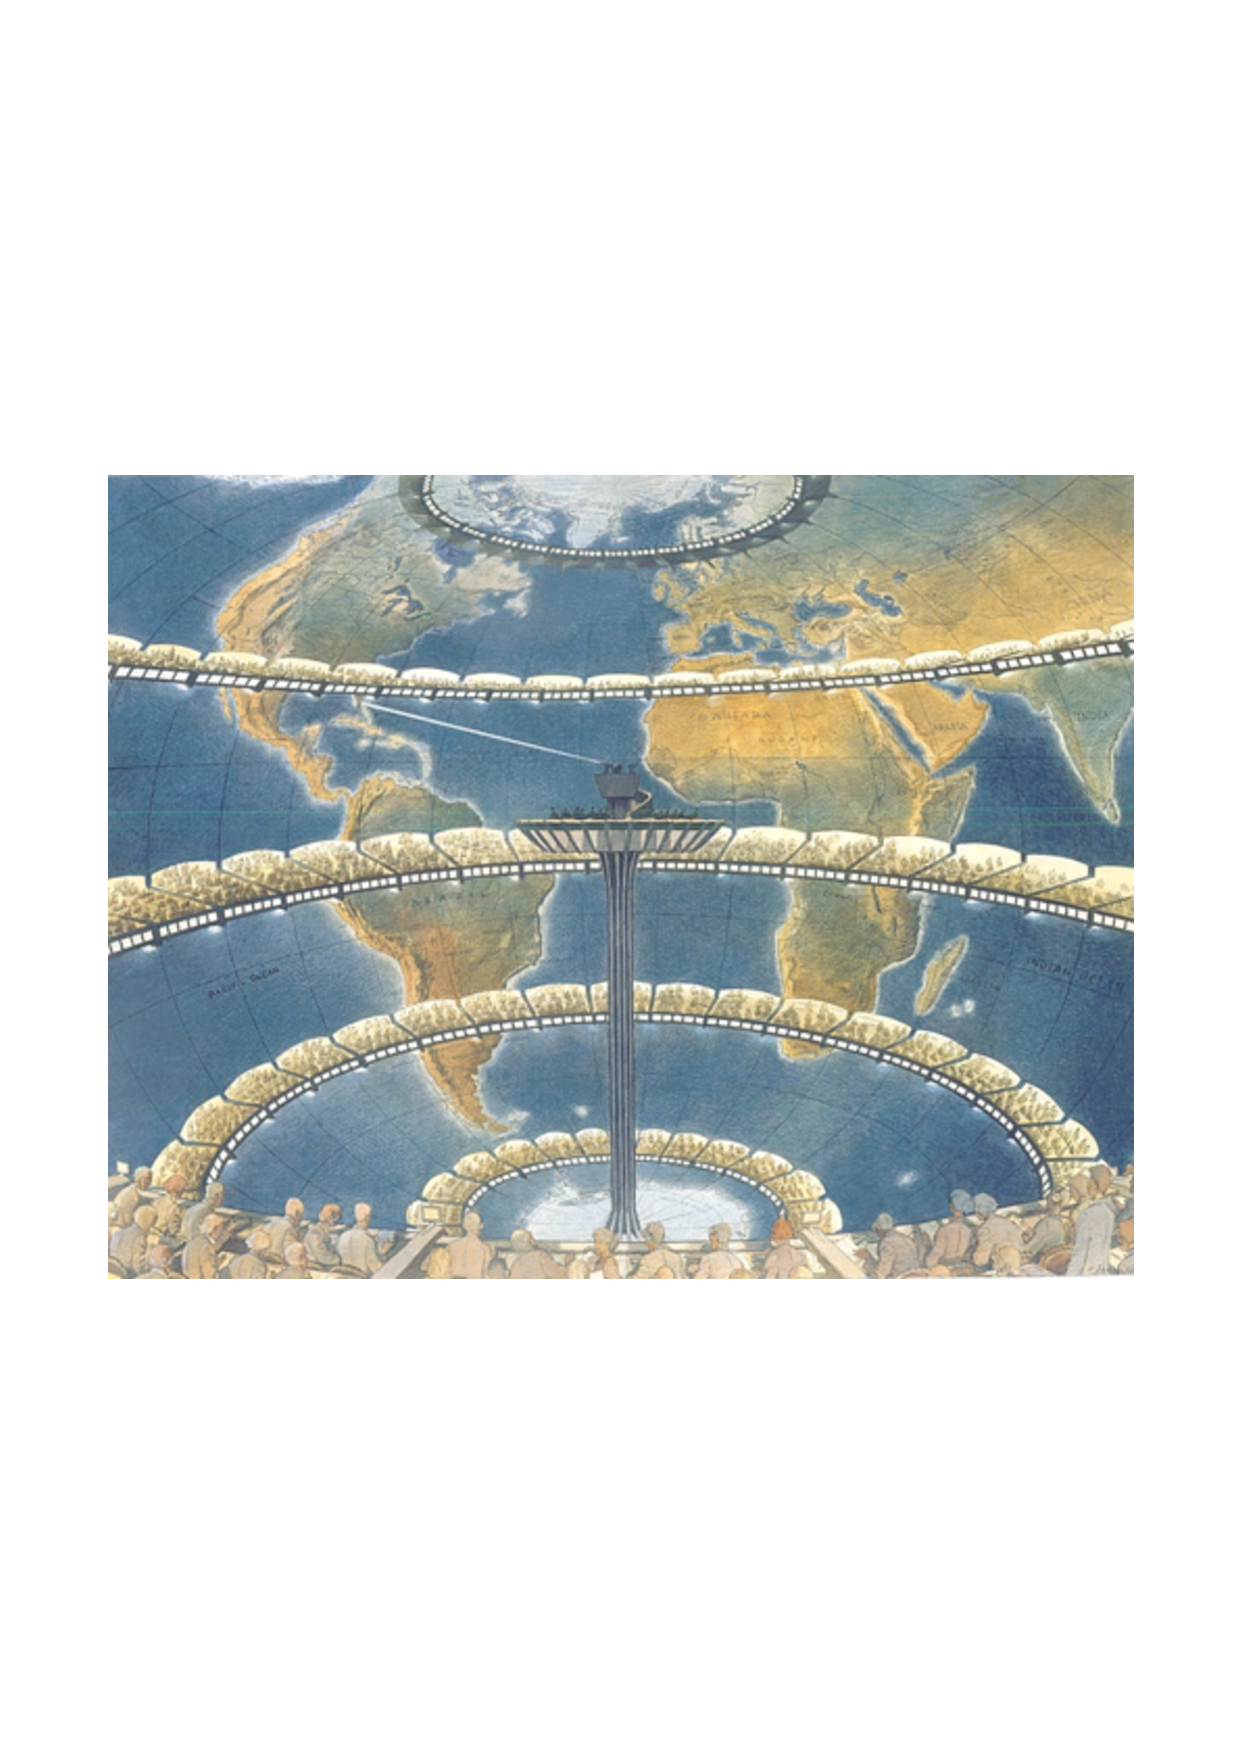
\includegraphics{image/SchuitenHD3.pdf}}
\end{frame}

\begin{frame}[t,fragile]{並列化とは何か}
  \begin{itemize}
    \setlength{\itemsep}{1em}
  \item 目的: シミュレーションをできる限り「短時間」で終了させる
    \begin{itemize}
      \item たとえ総CPU時間が伸びても「ターンアラウンド時間」を短かくしたい
      \item 一台のパソコンでは100年かかる計算を学位論文に間に合わせたい
      \item 今の100倍の精度の計算を同じ「実時間」で実行したい
    \end{itemize}
  \item 並列化とは
    \begin{enumerate}
    \item CPUの行なうべき仕事を複数の小さな仕事に分割
    \item それらを複数のCPUで同時実行
    \end{enumerate}
  \item うまく並列化を行なうために必要なこと
    \begin{enumerate}
    \item プログラムのどの部分をどのように並列化すればより効果的かを理解する
    \item 並列化を実装するにはどのようにプログラムを書けば良いかを理解する
    \end{enumerate}
  \end{itemize}
\end{frame}

\begin{frame}[t,fragile]{並列計算の原理}
  \begin{itemize}
    %\setlength{\itemsep}{1em}
  \item ノードは、互いに必要な情報を交換しながら、それぞれ異なる処理をしなければならない
  \item ノード毎に異なる指示(= プログラム)を与えるのは大変 (特にノード数が何万もの場合)
  \item 一つのプログラムでノード(ランクとも呼ばれる)毎に異なる指示を与えたい

    ⇒ SPMD (Single Program, Multiple Data streams)

    \resizebox{.9\textwidth}{!}{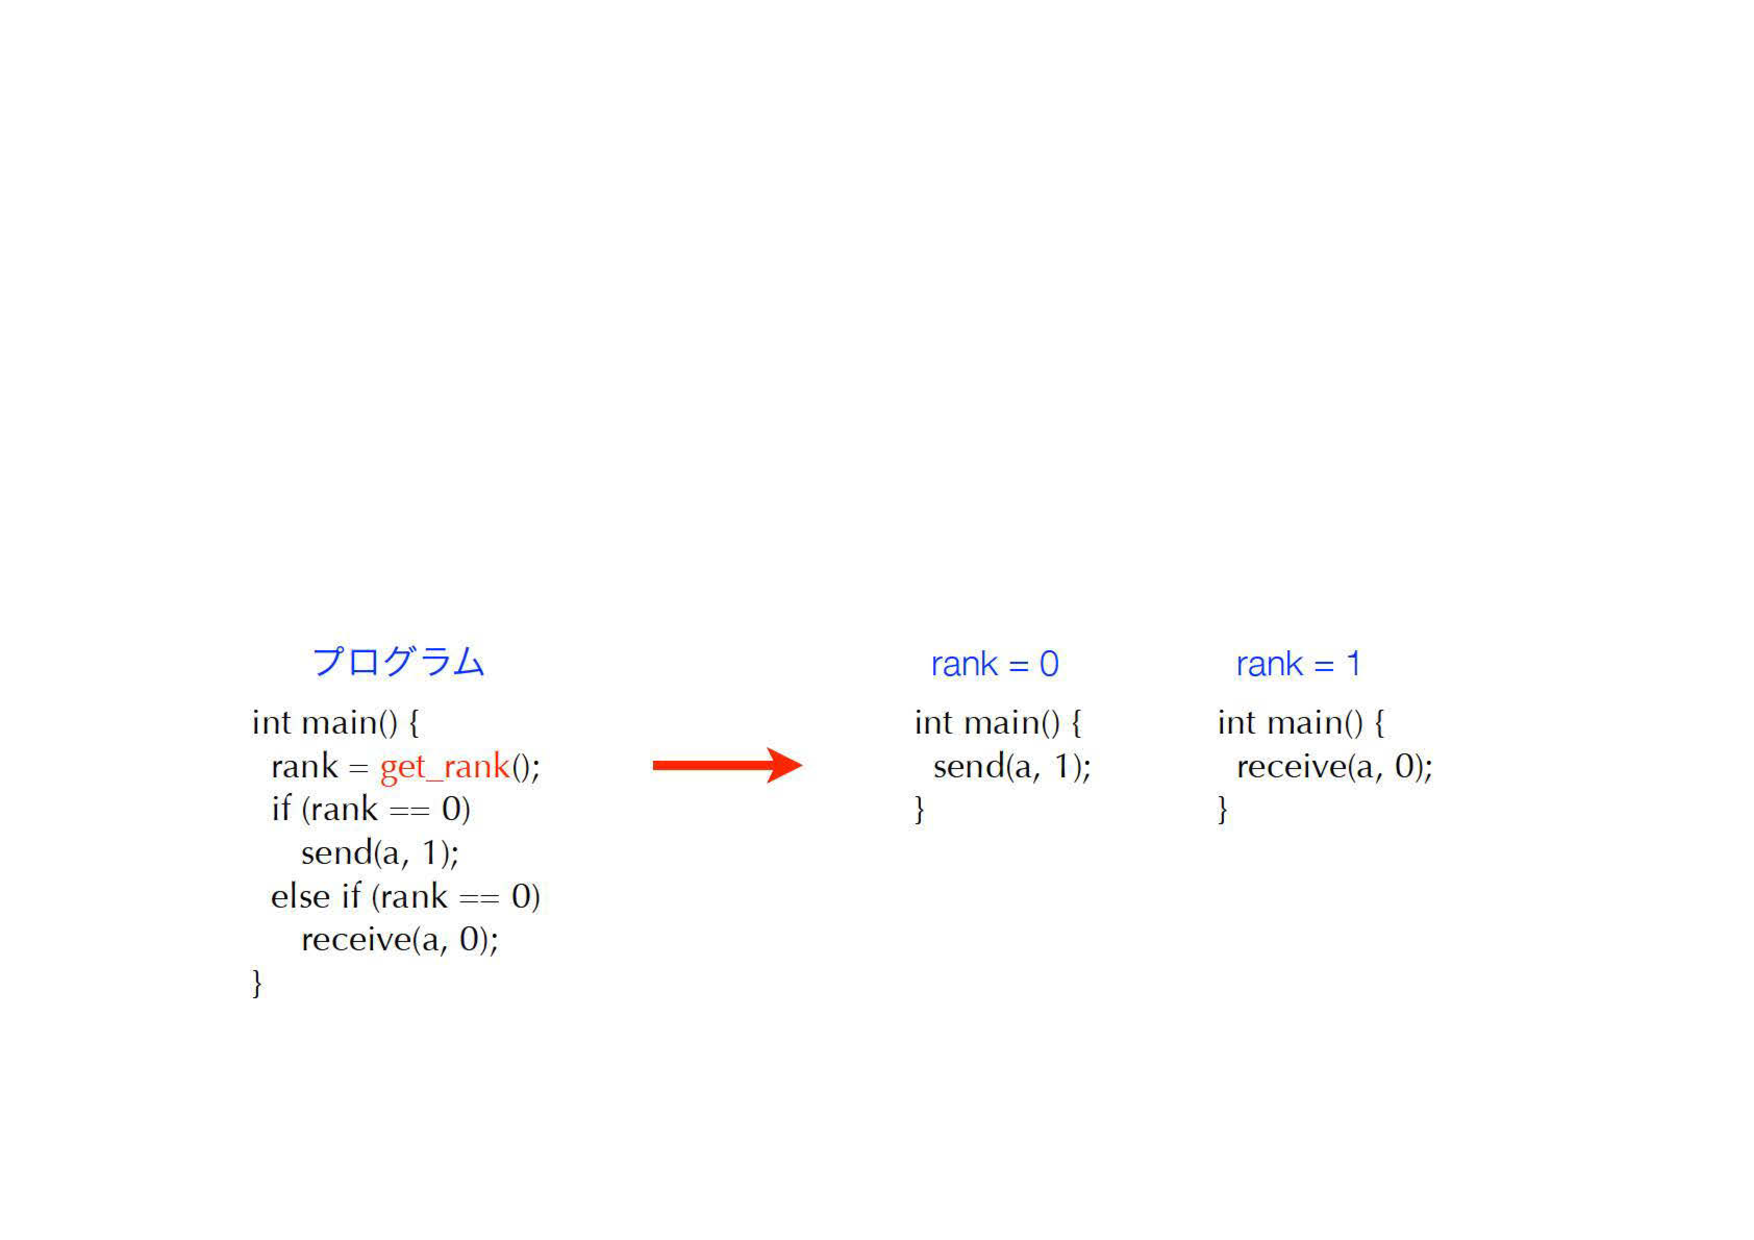
\includegraphics{image/spmd.pdf}}
  \end{itemize}
\end{frame}

\begin{frame}[t,fragile]{アムダール(Amdahl)の法則}
  \begin{itemize}
    \setlength{\itemsep}{1em}
  \item 並列化による全体の性能向上率
    \[
    P = \frac{1}{X+(1-X)/n}
    \]
    $X$: 並列化されていない部分の実行時間の割合, $n$: ノード数
  \item $X$を限りなく零にしないと高並列ではすぐに性能が頭打ちに
  \end{itemize}
  \vspace*{-0em}\hspace*{1em}\resizebox{0.5\textwidth}{!}{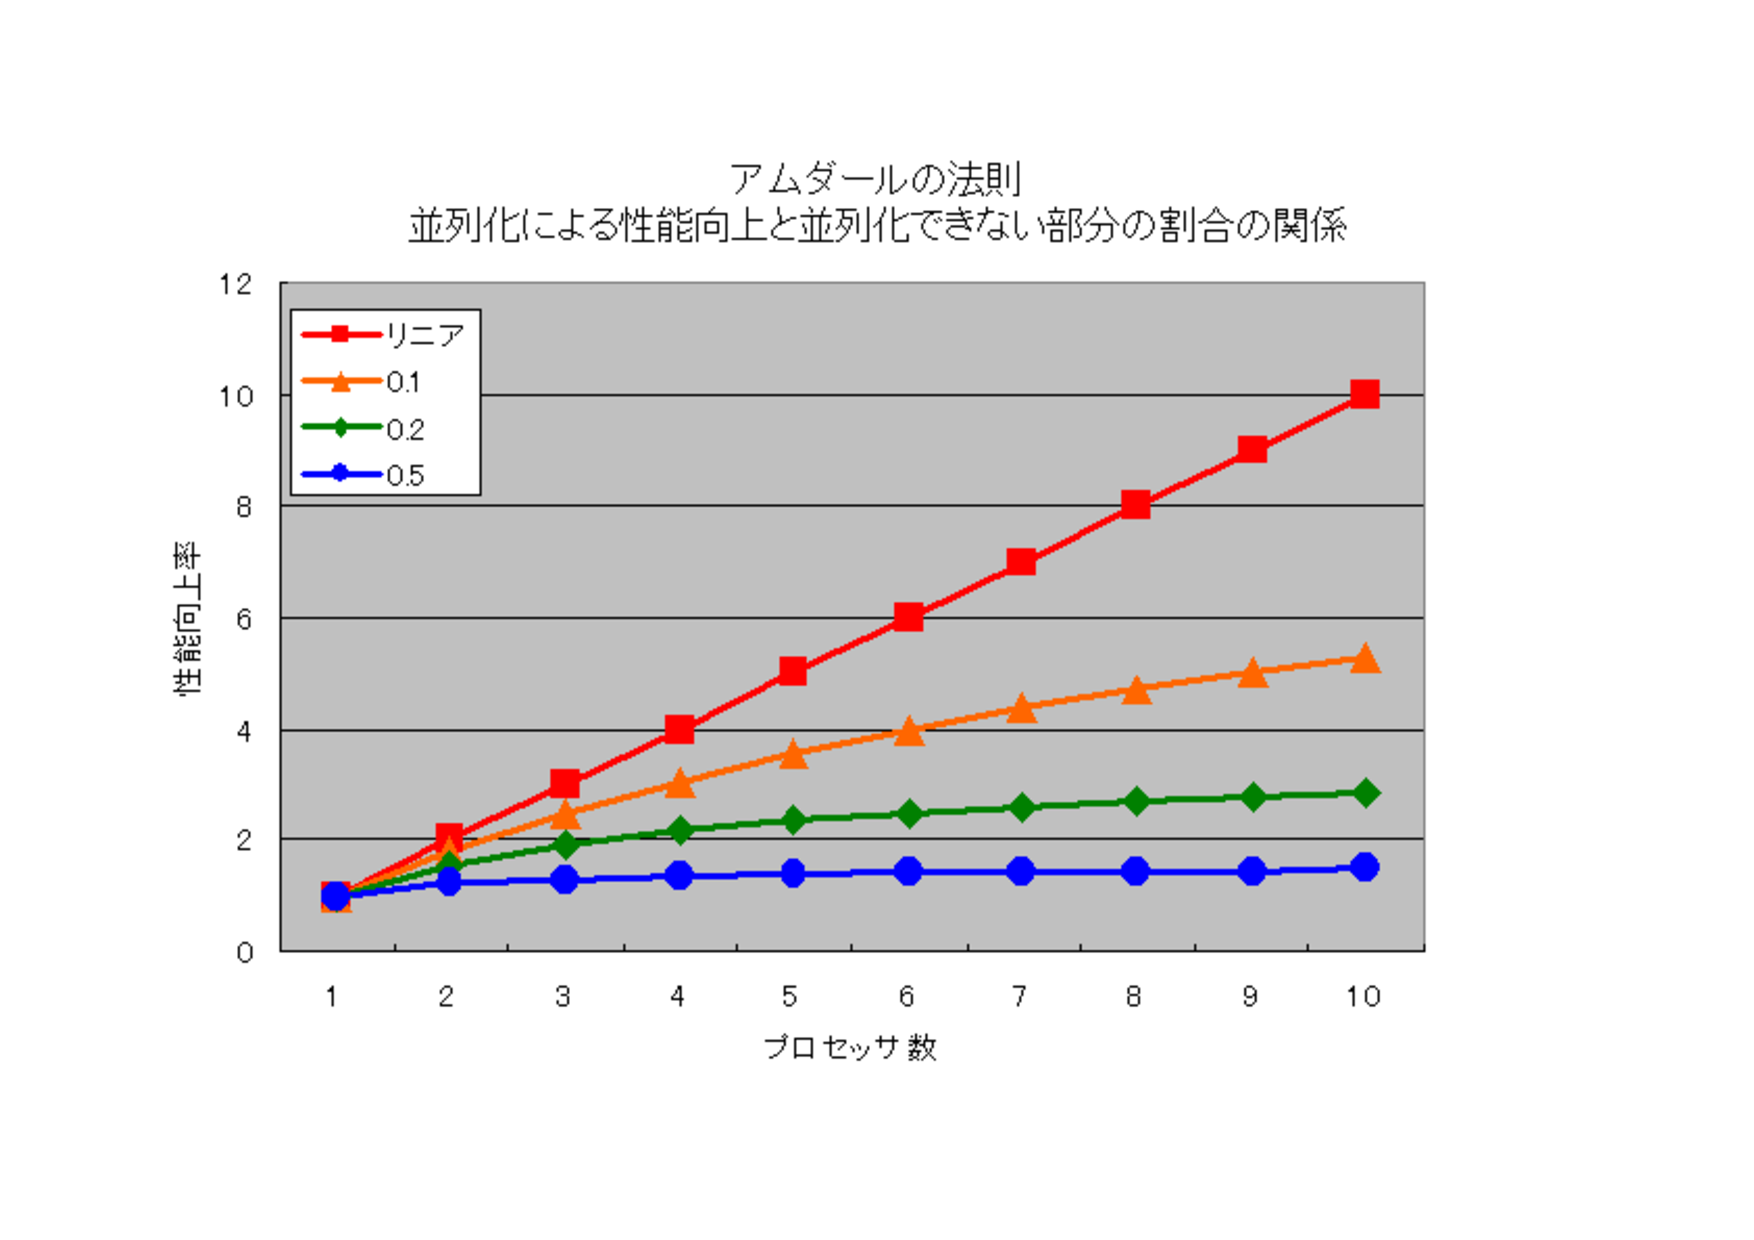
\includegraphics{image/Amdahl_law2.pdf}}
\end{frame}

\section{バッチキューシステム}

\begin{frame}[t,fragile]{バッチキューシステム}
  \begin{itemize}
    \setlength{\itemsep}{1em}
  \item 実習用計算機 photon
    \begin{itemize}
    \item ログインノード(2CPU, 12コア)+計算ノード(64CPU, 256コア)からなる「クラスタワークステーション」(並列計算機の一種)
    \item 普段{\tt ssh}して作業しているのはログインノード
    \end{itemize}
  \item バッチーキューシステム
    \begin{itemize}
    \item 長い(大きな)計算は計算ノードを使う
    \item 多数の計算ノードの割り振りを手でやるのは非効率的
    \item バッチキューシステムを使って、「ジョブ」を投入する
    \end{itemize}
  \item 詳しい説明は「システム利用マニュアル」({\tt ssh}ログイン時に表示されるメッセージ参照)を見ること
  \item photon は卒業まで継続して利用可 (希望すれば大学院でも)
  \end{itemize}
\end{frame}

\section{実習その8}

\begin{frame}[t,fragile]{EX8-1: 並列プログラムのコンパイルと実行}
  \begin{itemize}
    %\setlength{\itemsep}{1em}
  \item[8-1-1] \href{https://github.com/todo-group/computer-experiments/blob/master/exercise/hpc/pi_mpi.c}{exercise/hpc/pi\_mpi.c}は、長方形近似により$\pi$の計算を行う並列プログラムである。コンパイルして実行せよ
\begin{lstlisting}
$ mpicc pi_mpi.c -o pi_mpi -lm
$ mpirun -np 4 ./pi_mpi
\end{lstlisting}
  \item[8-1-2] {\tt pi\_mpi.c}のソースコードを解析せよ。{\tt nsteps}や並列数(上の例では4)を変えて、実行時間を測定せよ
  \end{itemize}
\end{frame}

\section{バージョン管理システムとは?}

\begin{frame}[t,fragile]{バージョン管理システムの必要性}
  \begin{itemize}
    \setlength{\itemsep}{1em}
  \item 広く行われている「ファイル管理」
    \begin{itemize}
    \item ファイル名・ディレクトリ名による管理

      (日付、人名、バージョン番号など)
    \item 手書きのログファイルによる記録
    \end{itemize}
  \item 問題点
    \begin{itemize}
    \item 記録を付け忘れる、記録を間違う、不完全な記録
    \item 人により命名規則がばらばら
    \item コンピュータ間でコピーを繰り返すと、どれを修正したか、どれが新しいか分からなくなる
    \item 同じバージョンを元に、別の人が独立に修正を行ってしまう

      (バージョンの分岐)
    \end{itemize}
  \end{itemize}
\end{frame}

\begin{frame}[t,fragile]{ありがちなパターン}
  \vspace*{-1.8em}
  \begin{center}
    \resizebox{0.93\textwidth}{!}{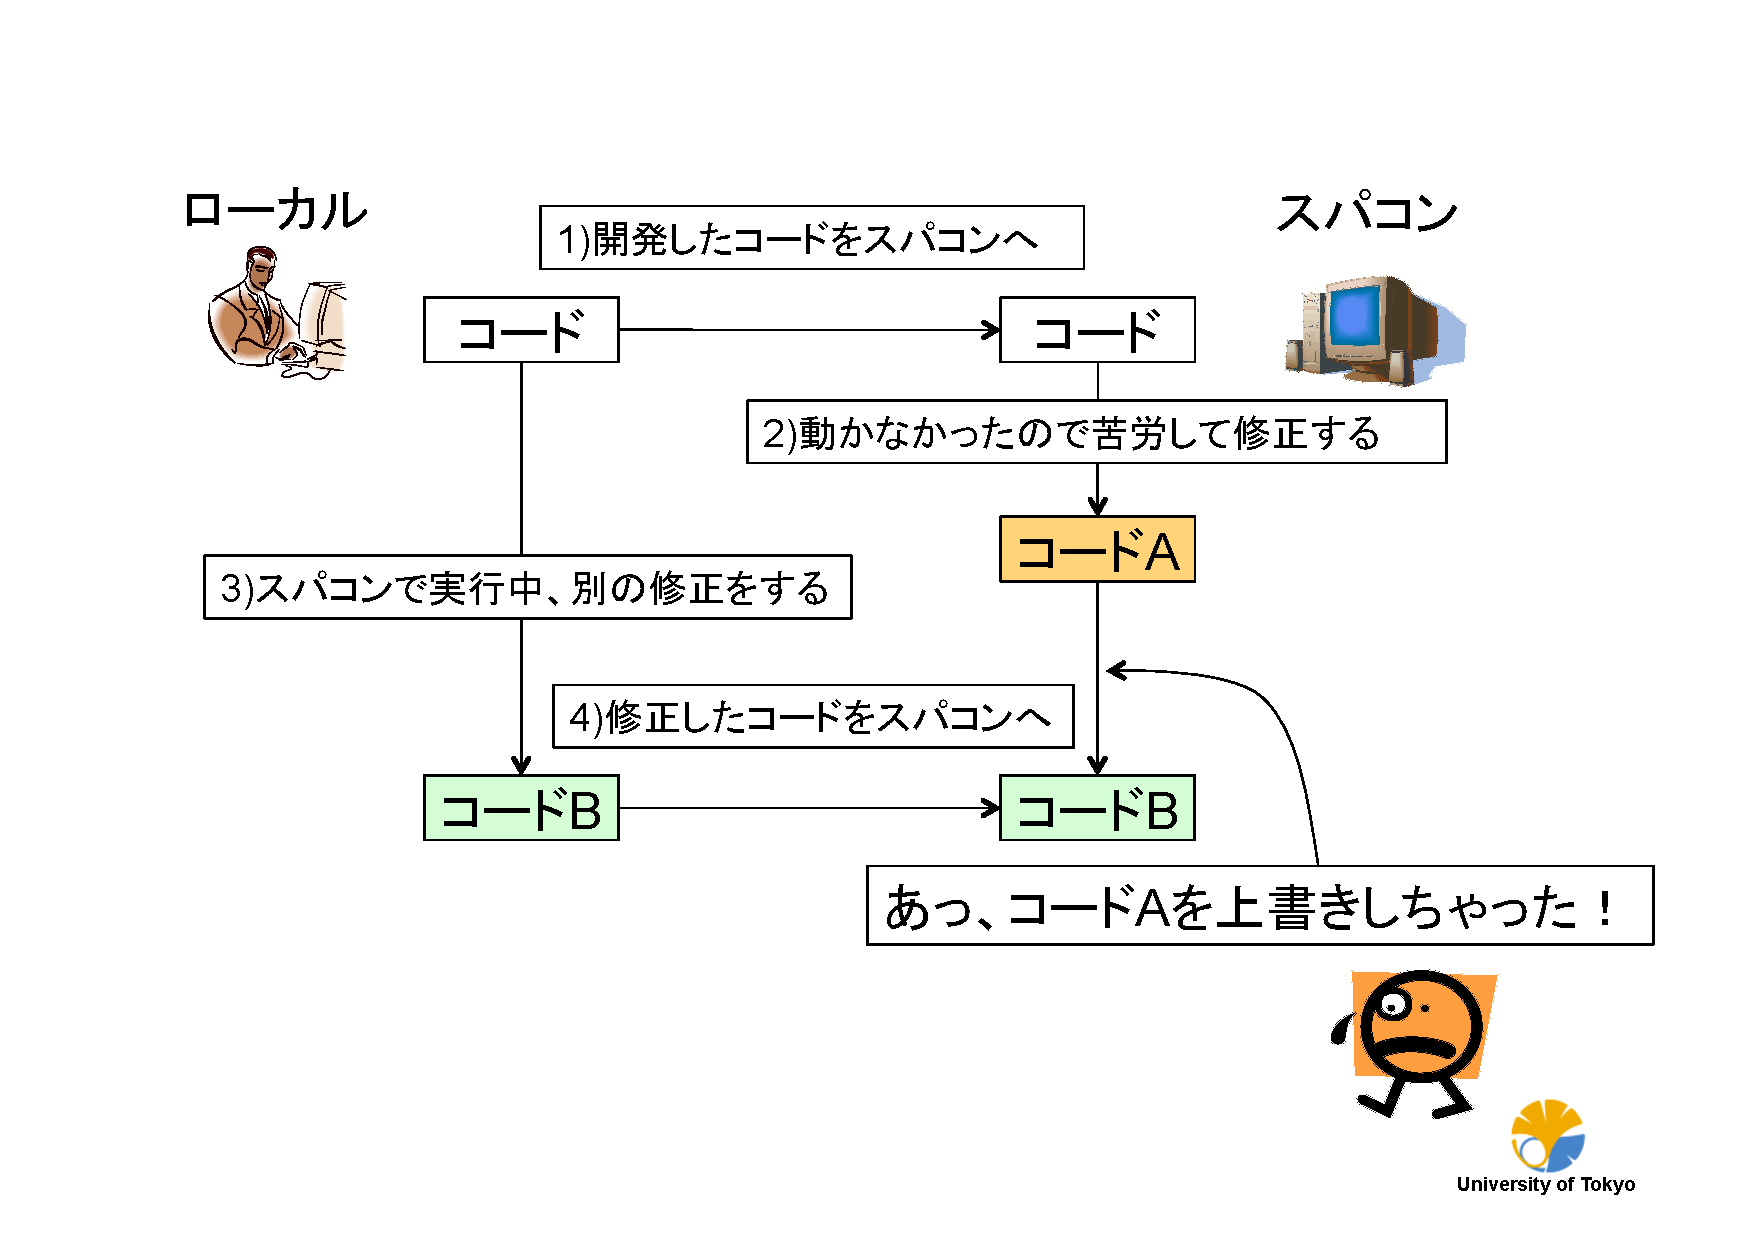
\includegraphics{image/vcs-bad.pdf}}
  \end{center}
  \vspace*{-2em}
  {\footnotesize (渡辺2013)}
\end{frame}

\begin{frame}[t,fragile]{バージョン管理システム(Version Control System)とは?}
  \begin{itemize}
    \setlength{\itemsep}{1em}
  \item ファイルの履歴をデータベース(リポジトリ)で一括管理するシステム
    \begin{itemize}
    \item 全ての修正履歴(差分)を保存
    \item 更新毎に一意なバージョン番号(リビジョン)を付与
    \item 任意のバージョン間の比較が可能
    \item もともとはプログラムのソースコードのためのシステム
    \item それ以外のファイル(例えば TeX ファイル)管理にも使える
    \end{itemize}
  \item チーム・分散環境での作業をサポート
    \begin{itemize}
    \item ネットワーク経由でファイルを check out/check in
    \item 複数箇所から同時に更新した場合に衝突を回避するしくみ
    \item ブランチ・マージ・タグの管理
    \item 一人で使っても複数人で使っても超便利
    \item 超優秀な(かつ超まじめな)秘書のようなもの (しかもタダ)
    \end{itemize}
  \end{itemize}
\end{frame}

\begin{frame}[t,fragile]{バージョン・ブランチ・マージ}
  \begin{center}\resizebox{!}{0.8\textheight}{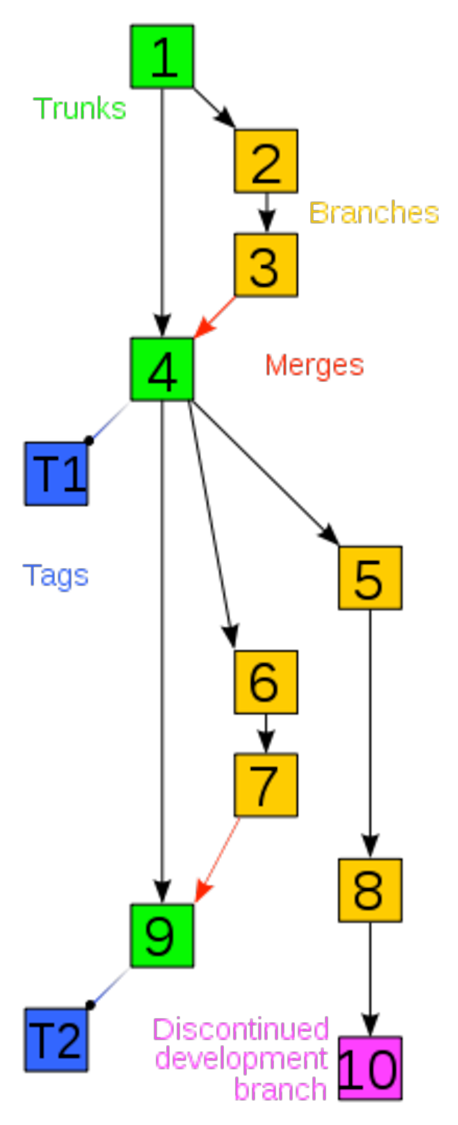
\includegraphics{image/revision.pdf}}\end{center}
\end{frame}

\begin{frame}[t,fragile]{バージョン管理を使うと}
  \vspace*{-1.8em}
  \begin{center}
    \resizebox{1.0\textwidth}{!}{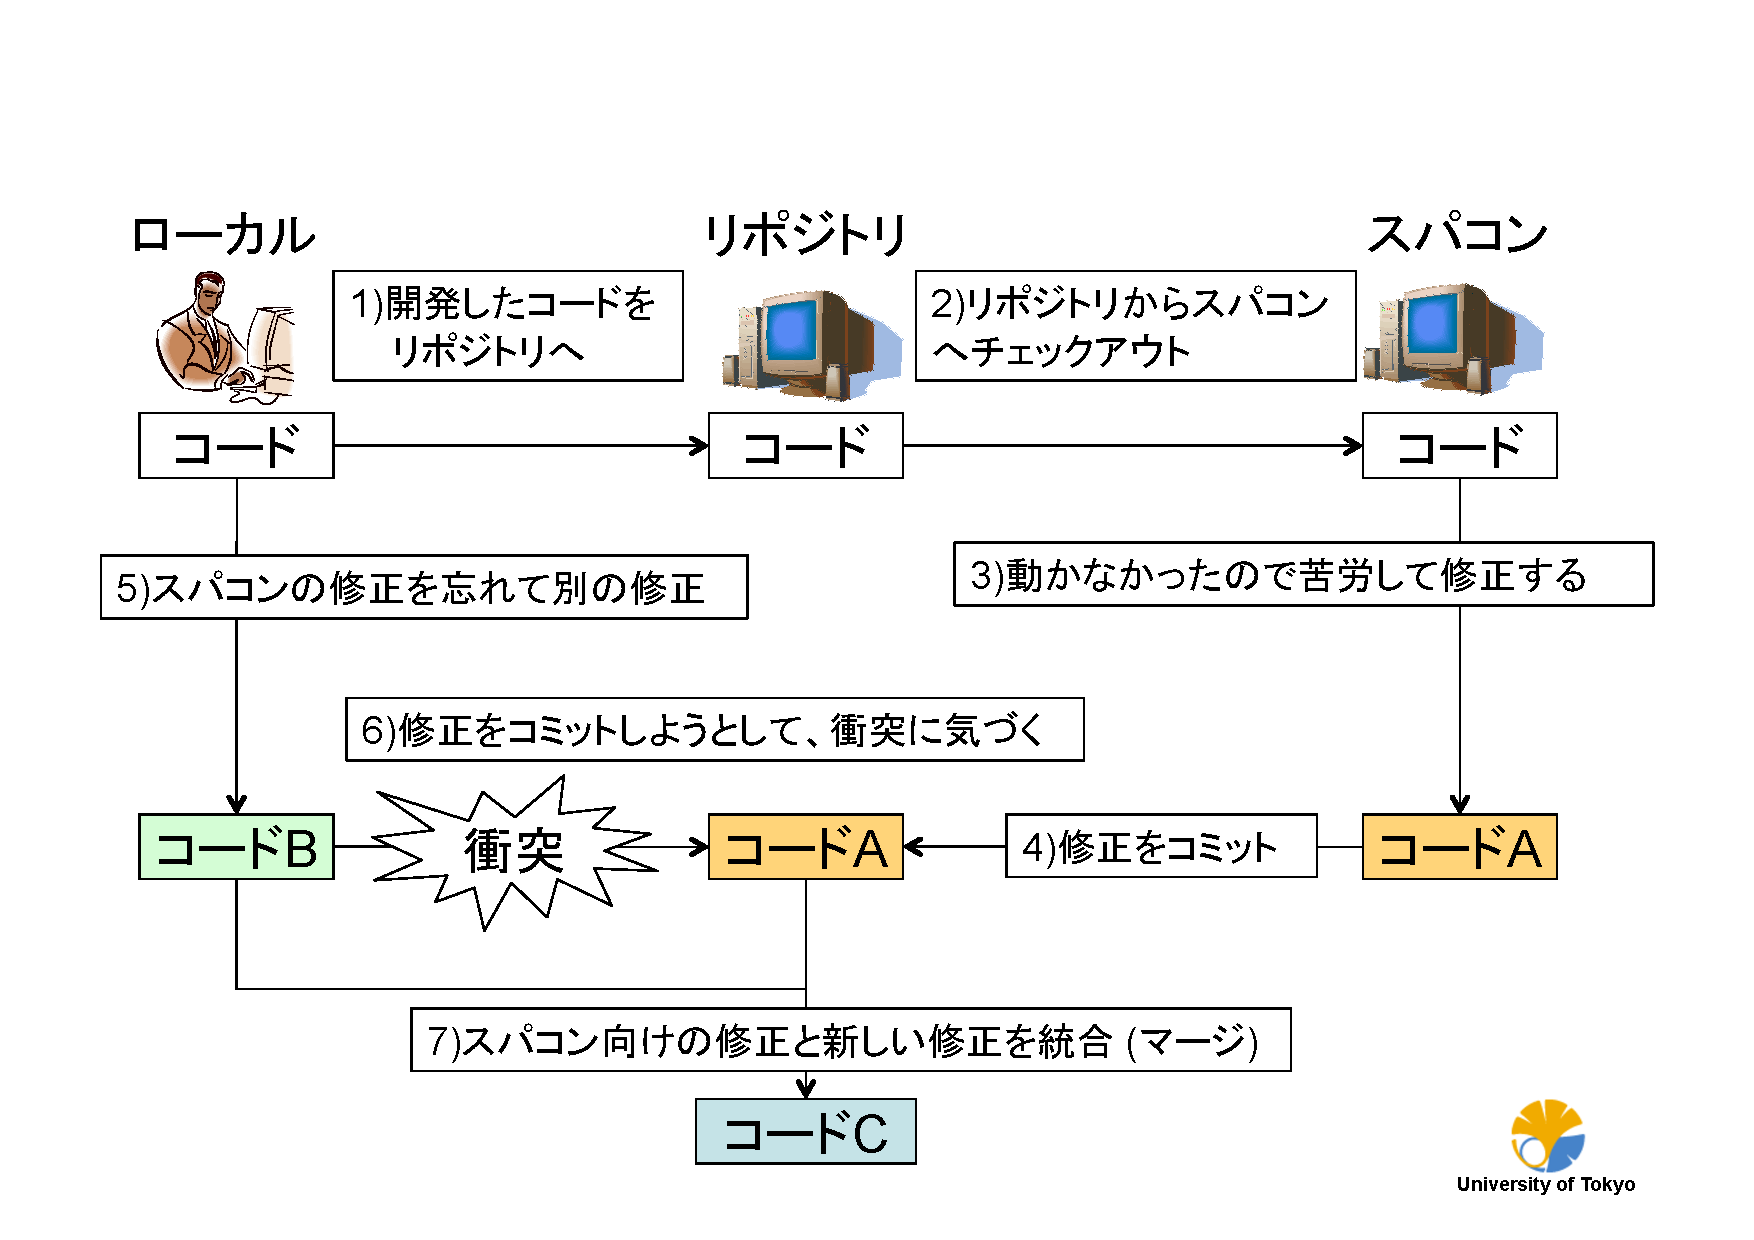
\includegraphics{image/vcs-good.pdf}}
  \end{center}
  \vspace*{-2em}
  {\footnotesize (渡辺2013)}
\end{frame}

\begin{frame}[t,fragile]{diff と patch}
  \begin{itemize}
    \setlength{\itemsep}{1em}
  \item {\tt diff}: 2つのテキストファイルの差分を出力するコマンド
    \begin{itemize}
    \item ファイル全体を保存するよりコンパクト
    \item 変更点を確認しやすい
      
      {\tt \$ \underline{diff -u file1.txt file2.txt > file.diff}}
    \end{itemize}
  \item {\tt patch}: {\tt diff}コマンドが生成した差分をファイルに適用するユーティリティー
    \begin{itemize}
    \item もとのファイルと差分から変更後のファイルを生成できる

      {\tt \$ \underline{patch < file.diff}}
    \end{itemize}
  \end{itemize}
\end{frame}

\begin{frame}[t,fragile]
  \frametitle{実習: diff \& patch (1)}
  \begin{itemize}
    %\setlength{\itemsep}{1em}
  \item 単一ファイルの例
\begin{lstlisting}
$ cp prologue.txt prologue-orig.txt
$ vi prologue.txt # prologue.txtを編集

$ diff -u prologue-orig.txt prologue.txt > prologue.diff
$ less prologue.diff # prologue.diffの中身を見てみる

$ mv prologue-orig.txt prologue.txt
$ patch < prologue.diff
$ less prologue.txt # prologue.txtの中身を確認
\end{lstlisting}
  \end{itemize}
\end{frame}

\begin{frame}[t,fragile]
  \frametitle{実習: diff \& patch (2)}
  \begin{itemize}
    %\setlength{\itemsep}{1em}
  \item ディレクトリ全体を扱う例
\begin{lstlisting}
$ cp -r vcs vcs.orig
# vcsの中のファイルを編集(ファイルの削除や追加も可)

$ diff -urN vcs.orig vcs > vcs.diff
$ less vcs.diff # vcs.diffの中身を見てみる

$ rm -rf vcs
$ mv vcs.orig vcs
$ patch -p0 < vcs.diff
# vcsの中身を確認
\end{lstlisting}
  \item diff と patch で差分の管理は可能になるが, 履歴は別に管理してお
    かなければならない
  \end{itemize}
\end{frame}

\section{Subversion入門}

\begin{frame}
  \frametitle{主なバージョン管理システム}
  \begin{itemize}
  \item BitKeeper - かつて Linux のカーネルのソース管理に使われていた
  \item CVS (Concurrent Versions System) - ネットワークでの利用を考慮とした初めてのバージョン管理システム. 以前はよく使われていた
  \item Git - 現在 Linux の開発に使われている. 分散型リポジトリ
  \item Mercurial - Git のライバル. 分散型リポジトリ
  \item SCCS (Source Code Control System) - 70年代にベル研で開発された世界初のバージョン管理システム. 現在は使われない
  \item {\color{red}Subversion} - CVSの改良版として開発された. 現在最もポピュラー? Mac OS X や多くの Linux には最初からインストールされている
  \end{itemize}
\end{frame}

\begin{frame}[t,fragile]{Subversionに関する資料}
  \begin{itemize}
    %\setlength{\itemsep}{1em}
  \item CVS/Subversionを使ったバージョン管理(前編:バージョン管理の基礎)
    \begin{itemize}
    \item \url{http://sourceforge.jp/magazine/08/09/09/1038233}
    \end{itemize}
  \item CVS/Subversionを使ったバージョン管理(後編:SVNを使ったバージョン管理)
    \begin{itemize}
      \item \url{http://sourceforge.jp/magazine/08/09/24/113215}
    \end{itemize}
  \item Subversion によるバージョン管理
    \begin{itemize}
      \item \url{http://svnbook.red-bean.com/index.ja.html}
    \end{itemize}
  \item 「Subversion によるバージョン管理」の読み方
    \begin{itemize}
      \item \url{http://exa.phys.s.u-tokyo.ac.jp/ja/members/wistaria/log/subversion-intro}
    \end{itemize}
  \item Gitを使いたい場合には、、、
    \begin{itemize}
      \item \href{http://www.cms-initiative.jp/ja/research-support/develop-support/how-to-publish/develop-apps/dt0l33/manage-version}{CMSIハンズオン - バージョン管理システム}
    \end{itemize}
  \end{itemize}
\end{frame}

\begin{frame}[t,fragile]{Subversionリポジトリ}
  \begin{columns}[T]
    \begin{column}{.7\textwidth}
      \begin{itemize}
        \setlength{\itemsep}{1em}
      \item ソースコードの全ての履歴を保存する「データベース」
      \item リポジトリからソースコードのチェックアウト
      \item リポジトリの実体は、ディスク上のディレクトリ
      \item リポジトリへのアクセス方法
        \begin{itemize}
        \item ssh によるアクセス: {\tt svn+ssh://ユーザ名@ホスト名/リポジトリ名}
        \item ネットワーク越しにアクセス可能
        \end{itemize}
      \end{itemize}
    \end{column}
    \begin{column}{.25\textwidth}
      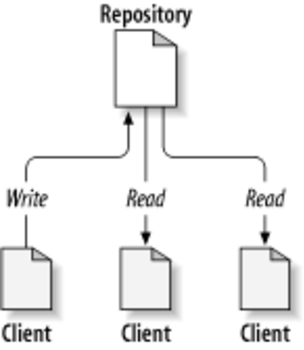
\includegraphics[width=\textwidth]{image/ch02dia1.pdf}
    \end{column}
  \end{columns}
\end{frame}

\begin{frame}[t,fragile]{URI (Uniform Resource Indicator)}
  \begin{itemize}
    \setlength{\itemsep}{1em}
  \item URI: (ネット上の)場所や名前を表す書式
    \begin{itemize}
    \item 例: URL (Uniform Resource Locator)

      {\footnotesize \url{https://wistaria@itc-lms.ecc.u-tokyo.ac.jp/lms/course/view.php?id=74564}}
    \item {\color{red}\tt https:} スキーム(scheme): プロトコル・アクセス方法を指定
    \item {\color{red}\tt wistaria@} ユーザ情報: ユーザ名(やパスワード)を指定
    \item {\color{red}\tt itc-lms.ecc.u-tokyo.ac.jp} ホスト名・サーバ名
    \item ``{\color{red}\tt //}''\ からホスト名までをオーソリティ(authority)と呼ぶ
    \item {\color{red}\tt /lms/course/view.php} パス名
    \item {\color{red}\tt ?iid=74564} クエリ(query): サーバへの指示や命令
  \end{itemize}
  \item SubversionのリポジトリのURIの例

    {\scriptsize \tt {\color{red} svn+ssh:}//{\color{blue} ce05151598@}cmp.phys.s.u-tokyo.ac.jp/home/ce05151598/svnroot}
  \end{itemize}
\end{frame}

\begin{frame}[t,fragile]{注意事項}
  \begin{itemize}
    %\setlength{\itemsep}{1em}
  \item 大きなバイナリファイル(pdf, exe, doc, tar.gz, zipなど)はなるべくsubversionで管理しない
    \begin{itemize}
      \item バイナリファイルはうまく差分が扱えない (マージできない)
    \end{itemize}
  \item チェックアウトしたディレクトリ「以外」でのファイルの編集は危い
    \begin{itemize}
      \item チェックアウト ⇒ ファイルをコピー ⇒ コピーしたファイルを変更 ⇒ チェックアウトしたディレクトリで svn update ⇒ 変更したファイルをチェックアウトしたディレクトリに戻す ⇒ svn commit ⇒ {\color{red}他の人の変更点を取り消してしまう!}
    \end{itemize}
  \item チェックアウトしたディレクトリには、管理用ディレクトリ'.svn'ができている
    \begin{itemize}
      \item チェックアウトしたオリジナルバージョンが保存されている
    \end{itemize}
  \item svn stat, svn diff はネットワークにつながってなくても使用可
  \end{itemize}
\end{frame}

\begin{frame}
  \frametitle{バージョン管理システムの欠点(面倒な点)}
  \begin{itemize}
  \item 修正前に最新の状態にアップデートしなければならない \\
   ⇒ 慣れると習慣になります
  \item 全ての修正を「コミット」しなければならない \\
    ⇒ 慣れると習慣になります
  \item 衝突(コンフリクト)が発生した時に対処しなければならない \\
    ⇒ 衝突に気づかずに修正してしまうほうが怖いです
  \item サーバのセットアップが面倒くさい \\
    ⇒ まずはホスティングサービス(github, sourceforge, bitbucket)を試してみましょう \\
    ⇒ まわりにいるプロ(?)に相談しましょう \\[.5em]
  \item バージョン管理システムを使うと作業効率が倍以上になる \\
    ⇒ {\color{red} 使わないと人生を半分損する}
  \end{itemize}
\end{frame}

\begin{frame}[t,fragile]{実習: Subversion (1)}
  \begin{itemize}
    %\setlength{\itemsep}{1em}
  \item 「ハンドブック 付録A バージョン管理システム」を読みながら以下の実習を行う
  \item リポジトリの作成 (photonにログインして作業)

    {\tt \$ \underline{svnadmin create \$HOME/svnroot}}
  \item リポジトリ内にフォルダを作成(iMacにもどって作業)

    {\tt \$~\underline{svn mkdir -m 'New folder' svn+ssh://.../svnroot/prog}}
  \item リポジトリの中をのぞいてみる

    {\tt \$ \underline{svn ls svn+ssh://.../svnroot}}

  \item リポジトリからのチェックアウト

    {\tt \$ cd \$HOME}
    
    {\tt \$ \underline{svn co svn+ssh://.../svnroot/prog}}

    ローカルに{\tt prog}ディレクトリが作成される(まだ中身は空)
  \end{itemize}
\end{frame}

\begin{frame}[t,fragile]{実習: Subversion (2)}
  \begin{itemize}
    %\setlength{\itemsep}{1em}
  \item ファイルの作成

    {\tt \$ \underline{cd prog}}
    
    {\tt \$ \underline{emacs main.c}}
  \item ファイルをsubverionの管理下に置く

    {\tt \$ \underline{svn add main.c}}
  \item 状態の確認

    {\tt \$ \underline{svn stat}}
  \item ファイルのコミット(サーバへの送信)

    {\tt \$ \underline{svn ci -m 'First version'}}
  \end{itemize}
\end{frame}

\begin{frame}[t,fragile]{実習: Subversion (3)}
  \begin{itemize}
    %\setlength{\itemsep}{1em}
  \item もう一つ別のディレクトリにチェックアウトしてみる

    {\tt \$ \underline{cd \$HOME}}
    
    {\tt \$ \underline{svn co svn+ssh://.../svnroot/prog other}}

    {\tt \$ \underline{cd other}}
    
  \item {\tt other}の下のファイルを修正、状態確認、コミット

    {\tt \$ \underline{emacs main.c}}

    {\tt \$ \underline{svn stat}}

    {\tt \$ \underline{svn ci -m 'Fixed a bug'}}
  \item {\tt \$HOME/prog}の下のファイルはそのまま
  \item 最新の状態にアップデート

    {\tt \$ \underline{cd \$HOME/prog}}

    {\tt \$ \underline{svn udpate}}
  \end{itemize}
\end{frame}

\begin{frame}[t,fragile]{実習: Subversion (4)}
  \begin{itemize}
    %\setlength{\itemsep}{1em}
  \item コミットしようとしたファイルがすでに他の人(or 他の場所)から更新されていたら
    \begin{itemize}
      \item {\color{red} コミットは失敗する}
    \end{itemize}
  \item 対処法
    \begin{itemize}
      \item まずは{\tt svn update}
      \item ファイル内の別の場所が更新されている場合: マージが成功するので、その後{\tt svn ci}
      \item ファイル内の同じ場所が更新されている場合: 衝突(コンフリクト)!

        ディレクトリ内に {\tt main.c.rXXX}, {\tt main.c.rYYY}, {\tt main.c.mine} ができる

        3つのファイルを参照しながら{\tt main.c}を編集し, {\tt svn resolved main.c}を実行した後、コミット
    \end{itemize}
  \end{itemize}
\end{frame}

\begin{frame}[t,fragile]{実習: Subversion (5)}
  \begin{itemize}
    \setlength{\itemsep}{1em}
  \item その他のコマンド
    \begin{itemize}
      \item svn mkdir dir
      \item svn move file1 file2
      \item svn copy file1 file2
      \item svn delete file
    \end{itemize}
  \item 変更履歴などを見る
    \begin{itemize}
      \item svn diff -r XXX {\ \# リビジョンXXXと現在の作業ファイル}
      \item svn diff -r XXX:YYY {\ \# 二つのリビジョン間}
      \item svn diff -c XXX {\ \# リビジョンXXX-1とXXX}
      \item svn log file
      \item svn annotate file {\ \# それぞれの行を誰がいつ変更したか}
    \end{itemize}
  \end{itemize}
\end{frame}


\end{document}
